%نام و نام خانوادگی:
%شماره دانشجویی: 
\مسئله{}
رایج است که روش \lr{Quality Function Deployment} را در مرحله استخراج نیازمندی‌ها استفاده می‌کنند.
\begin{enumerate}[a)]
	\item
این روش را تعریف کنید و خروجی‌های آن و همچنین نحوه به دست آمدن این خروجی‌ها را شرح دهید.
	
	\item
یکی از دام‌هایی که در استخراج نیازمندی‌ها برای تیم‌های نرم‌افزاری پیش می‌آید \lr{Requirement Creep} است. در مورد این دام تحقیق کنید و شرح دهید که چیست و چگونه می‌توان از آن اجتناب کرد. (۵ روش را ذکر کنید.)
\end{enumerate}

\پاسخ{
\begin{enumerate}[a)]
\item

\textbf{
تعریف روش \lr{Quality Function Deployment}\cite{geeksforgeeks}}

این روش که به اختصار QFD نامیده می‌شود، روند یا مجموعه ابزاری است که نیازمندی‌های مشتری را برای طراحان محصول مشخص کرده و این نیازمندی‌ها را در قالب ویژگی‌های مهندسی (\lr{Engineering Specifications}) و برنامه‌های پیاده‌سازی در می‌آورد. اصلی که در این روش بیشترین اهمیت را دارد برآورده شدن تمامی خواسته‌های مشتری در رابطه با محصول است. این روش ۴ گام اساسی دارد که عبارتند از:
\begin{itemize}
	\item برنامه‌ریزی محصول (\lr{Product Planning}) 
	
	در مرحله اول باید نیازمندی‌های مشتری به صورت مجموعه‌ای از نیازمندی‌هایِ طراحیِ اولویت‌بندی شده درآورده شود. محصولات رقیب و شناسایی تفاوت‌های آنها با محصول مورد نظر نیز در این مرحله انجام می‌شود. 
	
	\item برنامه‌ریزی قسمت‌ (\lr{Part Planning})
	
	در این بخش باید مشخص شود که به ازای هر نیازمندی مشتری، چه ویژگی‌هایی باید در محصول گنجانده شوند. برای مثال اگر هدف مشتری «رابط کاربری خوب» است، باید ویژگی‌های «طراحی زیبا» و «سهولت کارکرد» در لیست مشخصات قرار گیرند. 
	
	\item برنامه‌ریزی روند (\lr{Process Planning})

پس از مشخص شدن مشخصات محصول، باید روند موثر و کارآمدی برای پیاده‌سازی آنها پیدا شود.
	
	\item برنامه‌ریزی تولید (\lr{Production Planning})

در نهایت نیز پس از تعیین فرآيند، روند ساخت و ارائه محصول مورد بررسی قرار می‌گیرد.
\end{itemize}

\textbf{خروجی‌ها و نحوه محاسبه آنها}

یکی از مهم‌ترین ابزارهای مورد استفاده در روش \lr{QFD}، ابزار «خانه کیفیت (\lr{House of Quality})» است. با استفاده از این روش می‌توان تصمیم‌گیری آگاهانه‌تری در رابطه با نیازمندی‌های مشتریان انجام داد. این ابزار در واقع یک ماتریس است که رابطه بین نیازمندی‌های مشتری و توانایی محصول و سازنده در پاسخگویی به این نیازها را نشان می‌دهد. نمونه‌ای از این ماتریس در شکل زیر نشان‌ داده شده است.

\begin{figure}[h]
	\centering
	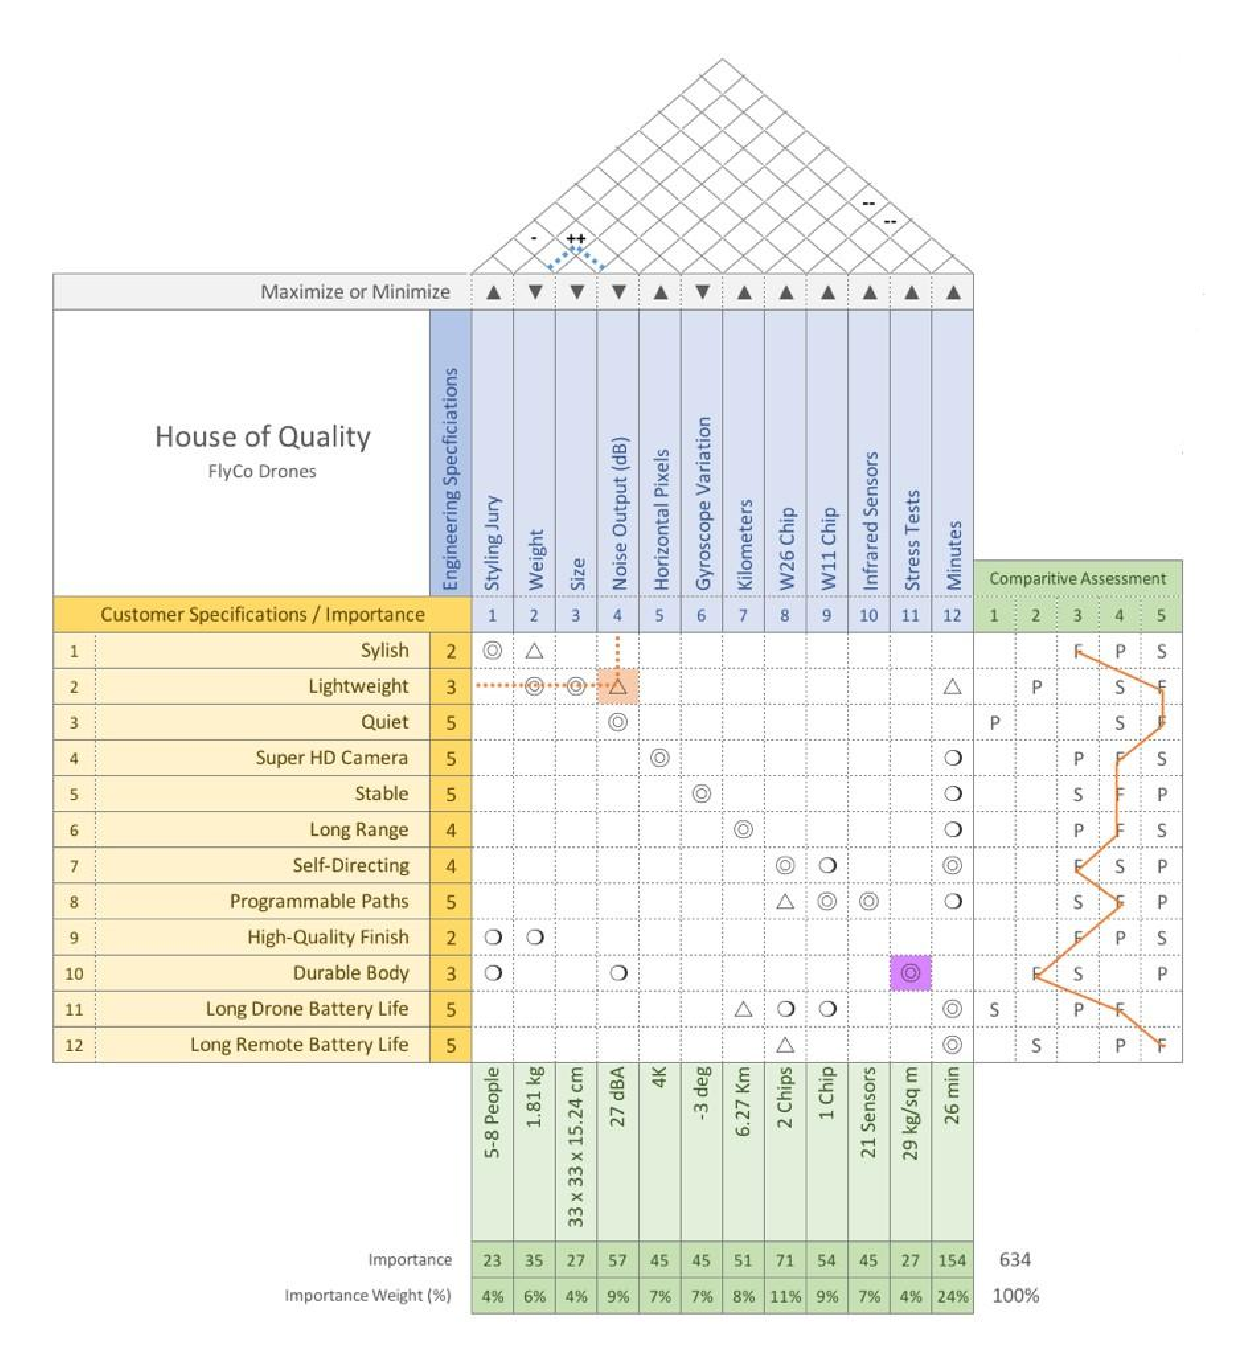
\includegraphics[scale=1]{figs/2-1}
\end{figure}

\begin{itemize}
\item
\lr{Customer Specification}: این بخش که در سمت چپ خانه قرار گرفته است، ویژگی‌های اولویت‌دار مشتری که بر روی آنها تمرکز زیادی دارد نشان می‌دهد. اعدادی که در سمت راست این ستون روبه‌روی ویژگی‌ها نوشته شده است نشان‌دهنده میزان اهمیت ویژگی مورد نظر در مقیاس ۱ تا ۵ است.

\item
\lr{Engineering Specification}: این بخش روش‌های مهندسی لازم برای اندازه‌گیری و پیش‌برد تولید را شامل می‌شود. 

\item
\lr{Specific Measurements}: برای تمامی ویژگی‌های کمیِ نیازمندِ اندازه‌گیری که در بخش \lr{Engineering Specification}، لازم است میزان اهمیت ویژگی همراه با واحد اندازه‌گیری آن در بخشی از خانه درج شود. این بخش همان پایین‌ترین بخش خانه است که با رنگ سبر مشخص شده است.

\item
\lr{Center Grid}: در بخش مرکزی میزان ارتباط بین هر ویژگی مد نظر مشتری و اندازه‌گیری‌های کمی مهندسی مشخص می‌شود. با توجه به راهنمای جدول که در شکل زیر نشان داده شده است، $\circledcirc$ نشان‌دهنده ارتباط قوی با وزن ۹ است. شکل دایره رابطه متوسط با وزن ۳ را نشان می‌دهد و در نهایت $\vartriangle$ نماینده وزن ۱ و رابطه ضعیف است.

\begin{figure}[h]
	\centering
	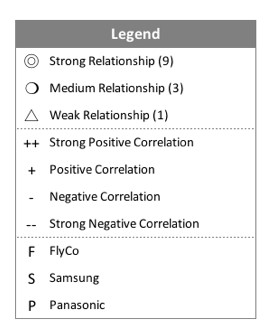
\includegraphics[scale=1.2]{figs/2-2}
\end{figure}

\end{itemize}

\end{enumerate}

\subsection*{مراجع}

\begin{latin}
	\begingroup
	\renewcommand{\section}[2]{}%
	
\begin{thebibliography}{9}
%   Check this for adding items: https://www.student.unsw.edu.au/how-do-i-cite-electronic-sources
	

	\bibitem{geeksforgeeks}
	17, P. (2020, August 17),
	\textit{Quality function deployment (QFD) in software quality},
	Accessed on 12/5/2022, 
	\url{https://www.geeksforgeeks.org/quality-function-deployment-qfd-in-software-quality/}

\end{thebibliography}
\endgroup
\end{latin}

}
\newpage
